\section{Introduction}
Dans ce chapitre, nous présenterons le corpus, les expérimentations et les différents choix effectués pour les tests.
\section{Corpus et expérimentations}
\subsection*{Le corpus}
\textbf{groove MIDI dataset}\\
\url{https://magenta.tensorflow.org/datasets/groove}\\\\
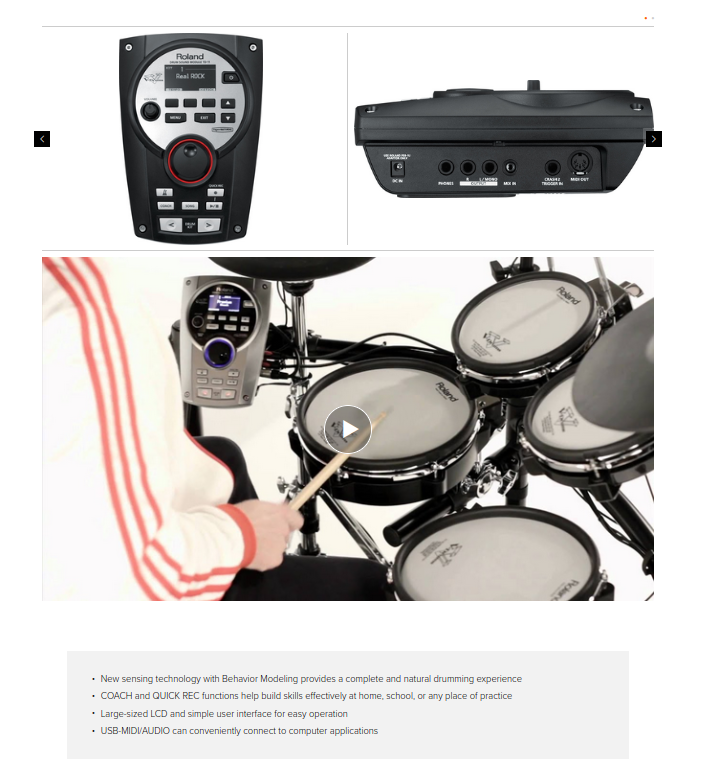
\includegraphics[height=60mm, width=60mm]{z_images/3_groove/roland_TD11.png}\\
Des batteurs pro ont été engagés pour jouer sur un roland td-11\\\\
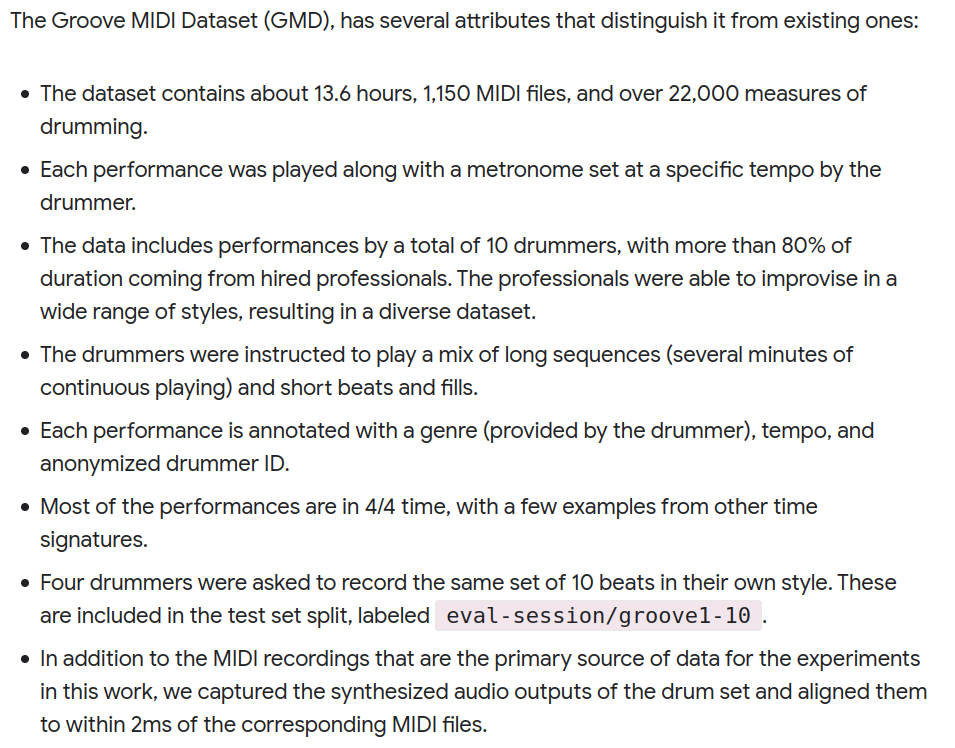
\includegraphics[height=80mm, width=110mm]{z_images/3_groove/dataset_how.png}\newpage{}
\textbf{Les métadatas :}\\\\
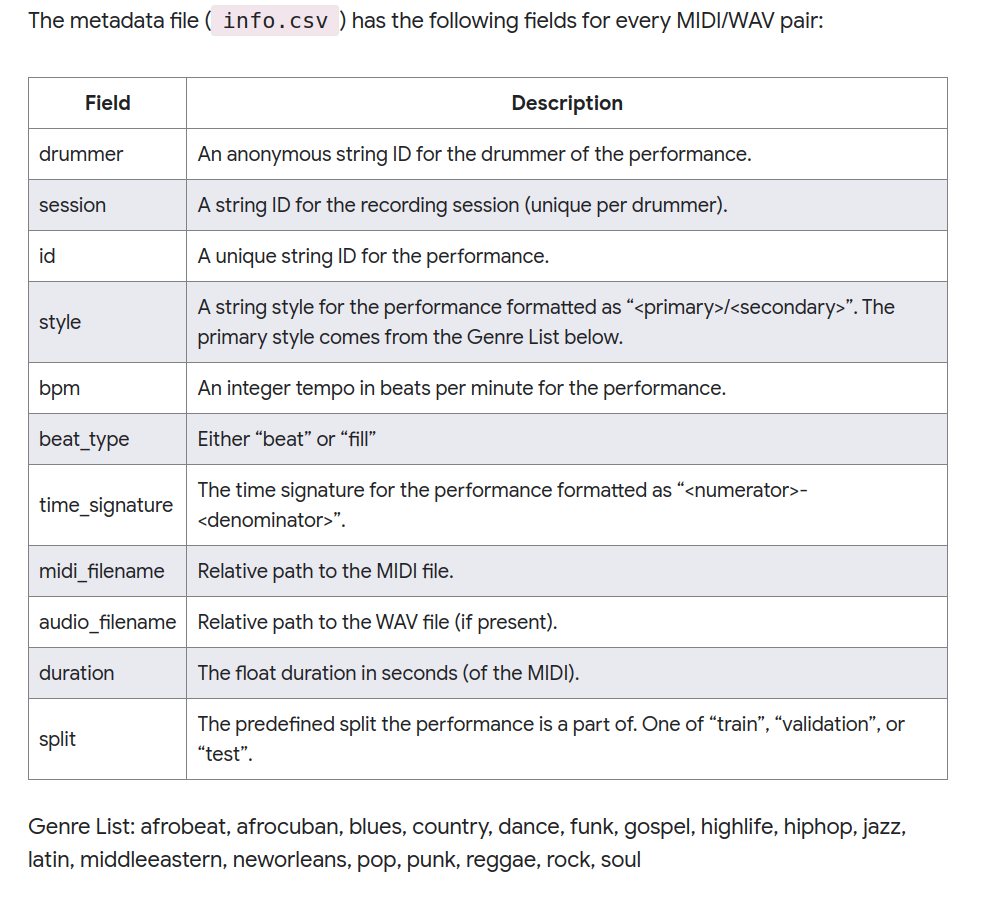
\includegraphics[height=85mm, 
width=100mm]{z_images/3_groove/csv_metadata_struct.png}\\
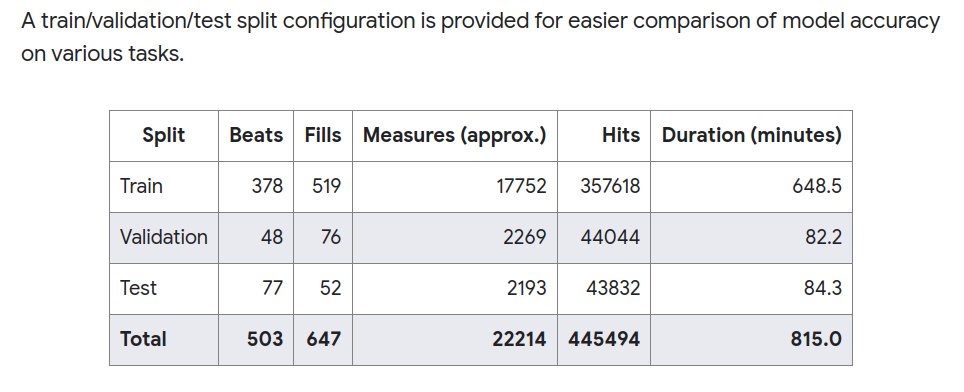
\includegraphics[height=50mm, width=120mm]{z_images/3_groove/train_validation_test.png}\\
Détails (entre autres tensorflow avec le dataset) à :
\url{https://magenta.tensorflow.org/datasets/groove#license}\\
écouter le dataset groove
\newpage
\subsection*{Les expérimentations}
\subsubsection{Comparaisons de transcriptions}
\textit{drummer\_01/session3 — 10\_rock-folk\_90\_beat\_4-4}\\\\
Fichier midi vers partition avec musescore $\Rightarrow$ Transcription manuelle\\
\includegraphics[height=20mm, width=50mm]{z_images/transcriptions_manuelles/0_prise_en_main/0_tests_drummer_01__session3/musescore_0.png}\ \ \ \ 
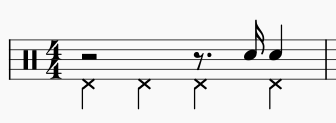
\includegraphics[height=20mm, width=55mm]{z_images/transcriptions_manuelles/0_prise_en_main/0_tests_drummer_01__session3/manuel_0.png}
\textit{drummer\_01/session3 — 10\_rock-folk\_90\_beat\_4-4}\\\\
Fichier midi vers partition avec musescore $\Rightarrow$ Transcription manuelle\\
\includegraphics[height=20mm, width=50mm]{z_images/transcriptions_manuelles/0_prise_en_main/0_tests_drummer_01__session3/musescore_0.png}\ \ \ \ 
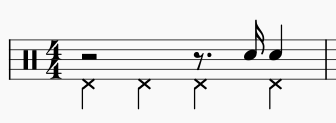
\includegraphics[height=20mm, width=55mm]{z_images/transcriptions_manuelles/0_prise_en_main/0_tests_drummer_01__session3/manuel_0.png}
\begin{itemize}
	\item Erreur d’indication de mesure ;
	\item Mauvaise transcription d’une noire.\\
\end{itemize}
La noire du 4ème temps se retrouve sur le premier temps de la mesure suivante et elle se transforme en un triolet de double croches dont seules les deux premières seraient jouées.\\\\
\textit{drummer\_01/session3 — 10\_rock-folk\_90\_beat\_4-4}\\\\
Fichier midi vers partition avec musescore $\Rightarrow$ Transcription manuelle\\
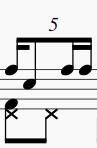
\includegraphics[height=20mm, width=15mm]{z_images/transcriptions_manuelles/0_prise_en_main/0_tests_drummer_01__session3/musescore_1.png}\ \ \ \ 
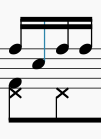
\includegraphics[height=20mm, width=15mm]{z_images/transcriptions_manuelles/0_prise_en_main/0_tests_drummer_01__session3/manuel_1.png}\\
\begin{itemize}
	\item Erreur de quantification : les doubles croches ont été interprétées en quintolet;\\
\end{itemize}
drummer\_01/session3 — 2\_jazz-swing\_185\_beat\_4-4\\\\
Fichier midi vers partition avec musescore $\Rightarrow$ Transcription manuelle\\
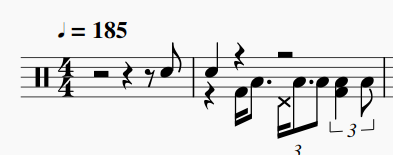
\includegraphics[height=25mm, width=60mm]{z_images/transcriptions_manuelles/0_prise_en_main/0_tests_drummer_01__session3/musescore_2.png}\ \ \ \ 
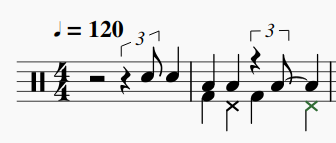
\includegraphics[height=25mm, width=55mm]{z_images/transcriptions_manuelles/0_prise_en_main/0_tests_drummer_01__session3/manuel_2.png}
\begin{itemize}
	\item L’indication de mesure est correcte mais tout a été décalé d’un temps car la première noire sur la caisse claire est jouée sur le 4ème temps et non sur le premier temps de la deuxième mesure comme l’indique la transcription de musescore.
	\item Les toms basses des 1er et 2ème temps de la mesure musescore auraient dû être sur les temps et non décalés d’une double croche vers la droite.\\
\end{itemize}
drummer\_01/session1 — 1\_funk\_80\_beat\_4-4\\\\
Fichier midi vers partition avec musescore $\Rightarrow$ Transcription manuelle\\
\includegraphics[height=25mm, width=40mm]{z_images/transcriptions_manuelles/0_prise_en_main/1_drummer_01__session1/musescore_0.png}\ \ \ \ 
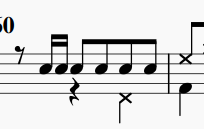
\includegraphics[height=25mm, width=40mm]{z_images/transcriptions_manuelles/0_prise_en_main/1_drummer_01__session1/Manuelle_0.png}
\begin{itemize}
	\item On dirait que lorsque certaines notes sont proches, elles se resserrent et suppriment celles qui aurait dû être sur le temps.\\
	\item Erreur d’indication de mesure ;
	\item Mauvaise transcription d’une noire.\\
\end{itemize}
La noire du 4ème temps se retrouve sur le premier temps de la mesure suivante et elle se transforme en un triolet de double croches dont seules les deux premières seraient jouées.\\\\
\textit{drummer\_01/session3 — 10\_rock-folk\_90\_beat\_4-4}\\\\
Fichier midi vers partition avec musescore $\Rightarrow$ Transcription manuelle\\
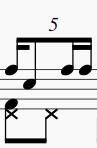
\includegraphics[height=20mm, width=15mm]{z_images/transcriptions_manuelles/0_prise_en_main/0_tests_drummer_01__session3/musescore_1.png}\ \ \ \ 
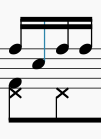
\includegraphics[height=20mm, width=15mm]{z_images/transcriptions_manuelles/0_prise_en_main/0_tests_drummer_01__session3/manuel_1.png}\\
\begin{itemize}
	\item Erreur de quantification : les doubles croches ont été interprétées en quintolet;\\
\end{itemize}
drummer\_01/session3 — 2\_jazz-swing\_185\_beat\_4-4\\\\
Fichier midi vers partition avec musescore $\Rightarrow$ Transcription manuelle\\
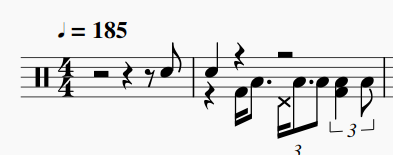
\includegraphics[height=25mm, width=60mm]{z_images/transcriptions_manuelles/0_prise_en_main/0_tests_drummer_01__session3/musescore_2.png}\ \ \ \ 
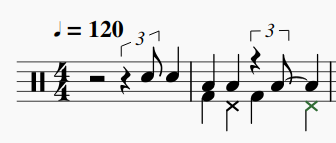
\includegraphics[height=25mm, width=55mm]{z_images/transcriptions_manuelles/0_prise_en_main/0_tests_drummer_01__session3/manuel_2.png}
\begin{itemize}
	\item L’indication de mesure est correcte mais tout a été décalé d’un temps car la première noire sur la caisse claire est jouée sur le 4ème temps et non sur le premier temps de la deuxième mesure comme l’indique la transcription de musescore.
	\item Les toms basses des 1er et 2ème temps de la mesure musescore auraient dû être sur les temps et non décalés d’une double croche vers la droite.\\
\end{itemize}
drummer\_01/session1 — 1\_funk\_80\_beat\_4-4\\\\
Fichier midi vers partition avec musescore $\Rightarrow$ Transcription manuelle\\
\includegraphics[height=25mm, width=40mm]{z_images/transcriptions_manuelles/0_prise_en_main/1_drummer_01__session1/musescore_0.png}\ \ \ \ 
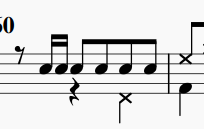
\includegraphics[height=25mm, width=40mm]{z_images/transcriptions_manuelles/0_prise_en_main/1_drummer_01__session1/Manuelle_0.png}
\begin{itemize}
	\item On dirait que lorsque certaines notes sont proches, elles se resserrent et suppriment celles qui aurait dû être sur le temps.\\
\end{itemize}
\textbf{Exemple avec des flas}\\\\
Fichier midi vers partition avec musescore :\\
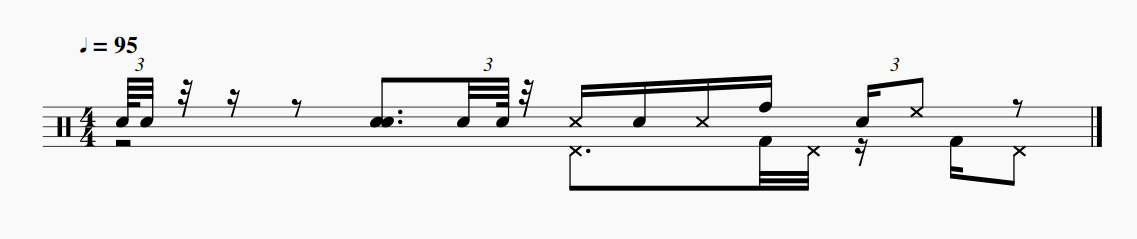
\includegraphics[height=30mm, width=120mm]{z_images/transcriptions_manuelles/1_transcriptions_flas/124_funk_95_fill_4-4_0.png}\\
Transcription manuelle :\\
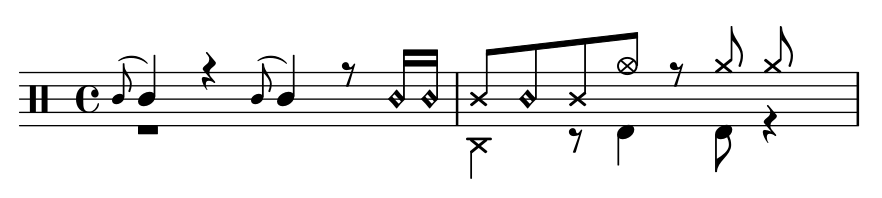
\includegraphics[height=20mm, width=90mm]{z_images/transcriptions_manuelles/1_transcriptions_flas/124_funk_95_fill_4-4_1_.png}\\
\subsubsection{Les tests unitaires}
\subsubsection{Le parsing avec squant}
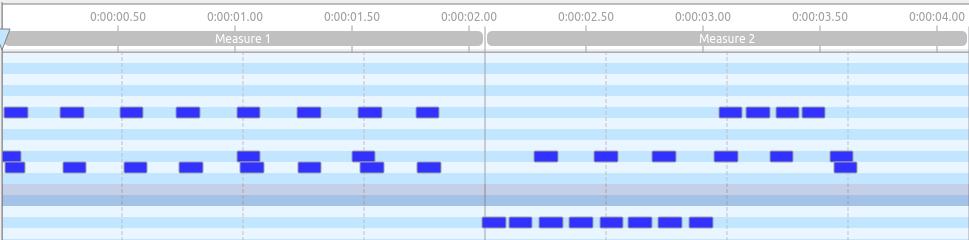
\includegraphics[height=80mm, width=160mm]{z_images/4_experimentations/input_parsing/midi_2bars_fill.png}
\subsubsection{Détails des expérimentations de bout en bout}
\textbf{Expérience 1 - 4/4 binaire}\\
\textbf{Partition de référence pour l’ouput}
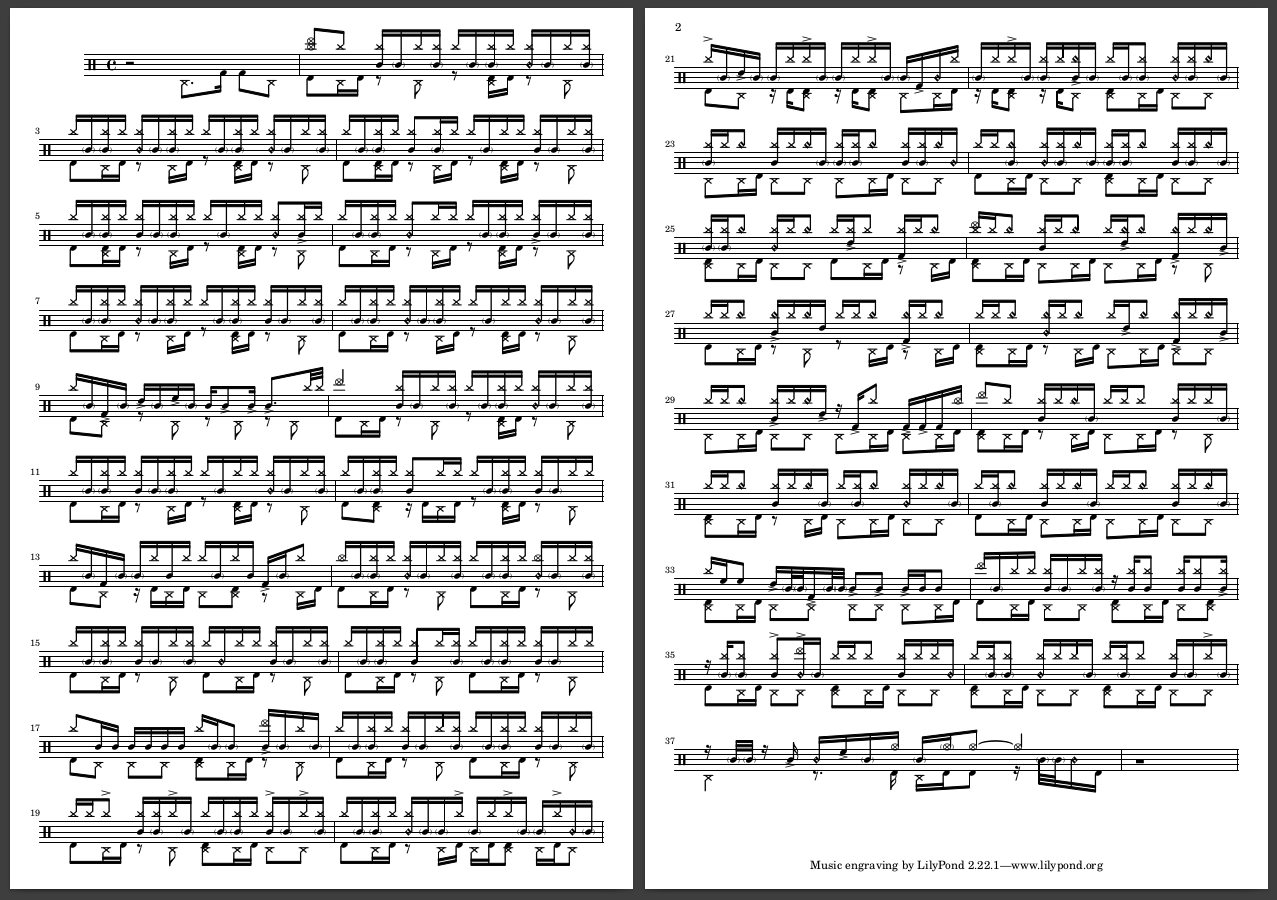
\includegraphics[height=120mm, width=160mm]{z_images/4_experimentations/experience_1/partition.png}
\textbf{Systèmes recherchés}
Textes :\\\\
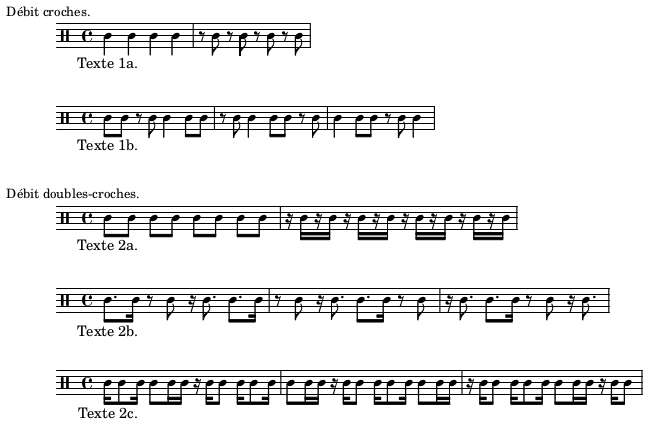
\includegraphics[height=70mm, width=95mm]{z_images/1_description_notation/systemes/0_textes_4-4_binaires.png}\\
Motifs :\\\\
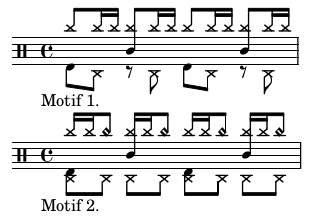
\includegraphics[height=30mm, width=40mm]{z_images/1_description_notation/systemes/1_motifs_4-4_binaires.png}\\\\
Systèmes résultants :\\\\
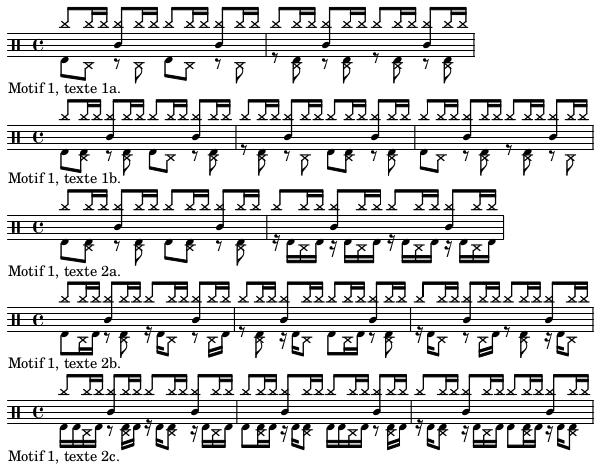
\includegraphics[height=75mm, width=85mm]{z_images/4_experimentations/experience_1/systeme_recherche_1.png}
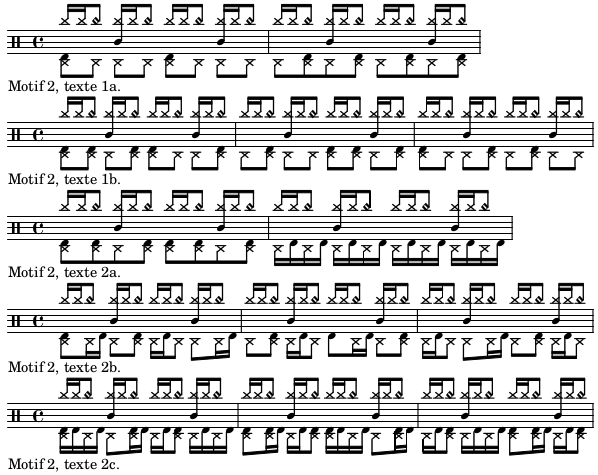
\includegraphics[height=75mm, width=85mm]{z_images/4_experimentations/experience_1/systeme_recherche_2.png}


\textbf{Représentation des systèmes en arbres de rythmes}

\resizebox{500pt}{!} {
	\Tree[.Motif\ 1\ +\ Texte\ 1a
	[.Mesure\ 1
	[.Temps\ 1 [rd\\bd ][ [rd\\pf ][rd ]]]
	[.Temps\ 2 [rd\\cc ][ [rd\\pf ][rd ]]]
	[.Temps\ 3 [rd\\bd ][ [rd\\pf ][rd ]]]
	[.Temps\ 4 [rd\\cc ][ [rd\\pf ][rd ]]] ]
	[.Mesure\ 2
	[.Temps\ 1 [rd ][ [rd\\bd\\pf ][rd ]]]
	[.Temps\ 2 [rd\\cc ][ [rd\\bd\\pf ][rd ]]]
	[.Temps\ 3 [rd ][ [rd\\bd\\pf ][rd ]]]
	[.Temps\ 4 [rd\\cc ][ [rd\\bd\\pf ][rd ]]] ]]}\\

\resizebox{500pt}{!} {
	\Tree[.Motif\ 1\ +\ Texte\ 1b
	[.Mesure\ 1
	[.Temps\ 1 [rd\\bd ][ [rd\\bd\\pf ][rd ]]]
	[.Temps\ 2 [rd\\cc ][ [rd\\bd\\pf ][rd ]]]
	[.Temps\ 3 [rd\\bd ][ [rd\\pf ][rd ]]]
	[.Temps\ 4 [rd\\cc ][ [rd\\bd\\pf ][rd ]]] ]
	[.Mesure\ 2
	[.Temps\ 1 [rd ][ [rd\\bd\\pf ][rd ]]]
	[.Temps\ 2 [rd\\cc ][ [rd\\pf ][rd ]]]
	[.Temps\ 3 [rd\\bd ][ [rd\\bd\\pf ][rd ]]]
	[.Temps\ 4 [rd\\cc ][ [rd\\bd\\pf ][rd ]]] ]
	[.Mesure\ 3
	[.Temps\ 1 [rd\\bd ][ [rd\\pf ][rd ]]]
	[.Temps\ 2 [rd\\cc ][ [rd\\bd\\pf ][rd ]]]
	[.Temps\ 3 [rd ][ [rd\\bd\\pf ][rd ]]]
	[.Temps\ 4 [rd\\cc ][ [rd\\pf ][rd ]]] ]]}\\

\resizebox{500pt}{!} {
	\Tree[.Motif\ 1\ +\ Texte\ 2a
	[.Mesure\ 1
	[.Temps\ 1 [rd\\bd ][ [rd\\bd\\pf ][rd ]]]
	[.Temps\ 2 [rd\\cc ][ [rd\\bd\\pf ][rd ]]]
	[.Temps\ 3 [rd\\bd ][ [rd\\bd\\pf ][rd ]]]
	[.Temps\ 4 [rd\\cc ][ [rd\\bd\\pf ][rd ]]] ]
	[.Mesure\ 2
	[.Temps\ 1 [rd ][bd ][rd\\pf ][rd\\bd ]]
	[.Temps\ 2 [rd\\cc ][bd ][rd\\pf ][rd\\bd ]]
	[.Temps\ 3 [rd ][bd ][rd\\pf ][rd\\bd ]]
	[.Temps\ 4 [rd\\cc ][bd ][rd\\pf ][rd\\bd ]] ]]}\\

\resizebox{500pt}{!} {
	\Tree[.Motif\ 1\ +\ Texte\ 2b
	[.Mesure\ 1
	[.Temps\ 1 [rd\\bd ][ [rd\\pf ][rd\\bd ]]]
	[.Temps\ 2 [rd\\cc ][ [rd\\bd\\pf ][rd ]]]
	[.Temps\ 3 [rd ][bd ][rd\\pf ][rd ]]
	[.Temps\ 4 [rd\\cc ][ [rd\\pf ][rd\\bd ]]] ]
	[.Mesure\ 2
	[.Temps\ 1 [rd\\ ][ [rd\\bd\\pf ][rd ]]]
	[.Temps\ 2 [rd\\cc ][bd ][rd\\pf ][rd ]]
	[.Temps\ 3 [rd\\bd ][ [rd\\pf ][rd\\bd ]]]
	[.Temps\ 4 [rd\\cc ][ [rd\\bd\\pf ][rd ]]] ]
	[.Mesure\ 3
	[.Temps\ 1 [rd ][bd ][rd\\pf ][rd ]]
	[.Temps\ 2 [rd\\cc ][ [rd\\pf ][rd\\bd ]]]
	[.Temps\ 3 [rd ][ [rd\\bd\\pf ][rd ]]]
	[.Temps\ 4 [rd\\cc ][bd ][rd\\pf ][rd ]]] ] }\\

\resizebox{500pt}{!} {
	\Tree[.Motif\ 1\ +\ Texte\ 2c
	[.Mesure\ 1
	[.Temps\ 1 [rd\\bd ][bd ][rd\\pf ][rd\\bd ]]
	[.Temps\ 2 [rd\\cc ][ [rd\\bd\\pf ][rd\\bd ]]]
	[.Temps\ 3 [rd ][bd ][rd\\bd\\pf ][rd ]]
	[.Temps\ 4 [rd\\cc ][bd ][rd\\pf ][rd\\bd ]] ]
	[.Mesure\ 2
	[.Temps\ 1 [rd\\bd ][ [rd\\bd\\pf ][rd\\bd ]]]
	[.Temps\ 2 [rd\\cc ][bd ][rd\\bd\\pf ][rd ]]
	[.Temps\ 3 [rd\\bd ][bd ][rd\\pf ][rd\\bd ]]
	[.Temps\ 4 [rd\\cc ][ [rd\\bd\\pf ][rd\\bd ]]] ]
	[.Mesure\ 3
	[.Temps\ 1 [rd ][bd ][rd\\bd\\pf ][rd ]]
	[.Temps\ 2 [rd\\cc ][bd ][rd\\pf ][rd\\bd ]]
	[.Temps\ 3 [rd\\bd ][ [rd\\bd\\pf ][rd\\bd ]]]
	[.Temps\ 4 [rd\\cc ][bd ][rd\\bd\\pf ][rd ]]] ] }\\\\

\textbf{Séparation des voix}
Motif\ 1\ +\ Texte\ 1a\\\\
\textit{Voix haute}\\
\resizebox{500pt}{!} {
	\Tree[.Motif\ 1\ +\ Texte\ 1a
	[.Mesure\ 1
	[.Temps\ 1 [rd ][ [rd ][rd ]]]
	[.Temps\ 2 [rd\\cc ][ [rd ][rd ]]]
	[.Temps\ 3 [rd ][ [rd ][rd ]]]
	[.Temps\ 4 [rd\\cc ][ [rd ][rd ]]] ]
	[.Mesure\ 2
	[.Temps\ 1 [rd ][ [rd ][rd ]]]
	[.Temps\ 2 [rd\\cc ][ [rd ][rd ]]]
	[.Temps\ 3 [rd ][ [rd ][rd ]]]
	[.Temps\ 4 [rd\\cc ][ [rd ][rd ]]] ]]}\\

\textit{Voix basse}\\
\resizebox{500pt}{!} {
	\Tree[.Motif\ 1\ +\ Texte\ 1a
	[.Mesure\ 1
	[.Temps\ 1 [bd ][ [pf ][t ]]]
	[.Temps\ 2 [t ][ [pf ][t ]]]
	[.Temps\ 3 [bd ][ [pf ][t ]]]
	[.Temps\ 4 [t ][ [pf ][t ]]] ]
	[.Mesure\ 2
	[.Temps\ 1 [t ][ [bd\\pf ][t ]]]
	[.Temps\ 2 [t ][ [bd\\pf ][t ]]]
	[.Temps\ 3 [t ][ [bd\\pf ][t ]]]
	[.Temps\ 4 [t ][ [bd\\pf ][t ]]] ]]}\\

Motif\ 1\ +\ Texte\ 1b\\\\
\textit{Voix haute}\\
\resizebox{500pt}{!} {
	\Tree[.Motif\ 1\ +\ Texte\ 1b
	[.Mesure\ 1
	[.Temps\ 1 [rd ][ [rd ][rd ]]]
	[.Temps\ 2 [rd\\cc ][ [rd ][rd ]]]
	[.Temps\ 3 [rd ][ [rd ][rd ]]]
	[.Temps\ 4 [rd\\cc ][ [rd ][rd ]]] ]
	[.Mesure\ 2
	[.Temps\ 1 [rd ][ [rd ][rd ]]]
	[.Temps\ 2 [rd\\cc ][ [rd ][rd ]]]
	[.Temps\ 3 [rd ][ [rd ][rd ]]]
	[.Temps\ 4 [rd\\cc ][ [rd ][rd ]]] ]
	[.Mesure\ 3
	[.Temps\ 1 [rd ][ [rd ][rd ]]]
	[.Temps\ 2 [rd\\cc ][ [rd ][rd ]]]
	[.Temps\ 3 [rd ][ [rd ][rd ]]]
	[.Temps\ 4 [rd\\cc ][ [rd ][rd ]]] ]]}\\

\textit{Voix basse}\\
\resizebox{500pt}{!} {
	\Tree[.Motif\ 1\ +\ Texte\ 1b
	[.Mesure\ 1
	[.Temps\ 1 [bd ][ [bd\\pf ][t ]]]
	[.Temps\ 2 [t ][ [bd\\pf ][t ]]]
	[.Temps\ 3 [bd ][ [pf ][t ]]]
	[.Temps\ 4 [t ][ [bd\\pf ][t ]]] ]
	[.Mesure\ 2
	[.Temps\ 1 [t ][ [bd\\pf ][t ]]]
	[.Temps\ 2 [t ][ [pf ][t ]]]
	[.Temps\ 3 [bd ][ [bd\\pf ][t ]]]
	[.Temps\ 4 [t ][ [bd\\pf ][t ]]] ]
	[.Mesure\ 3
	[.Temps\ 1 [bd ][ [pf ][t ]]]
	[.Temps\ 2 [t ][ [bd\\pf ][t ]]]
	[.Temps\ 3 [t ][ [bd\\pf ][t ]]]
	[.Temps\ 4 [t ][ [pf ][t ]]] ]]}\\

Motif\ 1\ +\ Texte\ 2a\\\\
\textit{Voix haute}\\
\resizebox{500pt}{!} {
	\Tree[.Motif\ 1\ +\ Texte\ 2a
	[.Mesure\ 1
	[.Temps\ 1 [rd ][ [rd ][rd ]]]
	[.Temps\ 2 [rd\\cc ][ [rd ][rd ]]]
	[.Temps\ 3 [rd ][ [rd ][rd ]]]
	[.Temps\ 4 [rd\\cc ][ [rd ][rd ]]] ]
	[.Mesure\ 2
	[.Temps\ 1 [rd ][t ][rd ][rd ]]
	[.Temps\ 2 [rd\\cc ][t ][rd ][rd ]]
	[.Temps\ 3 [rd ][t ][rd ][rd ]]
	[.Temps\ 4 [rd\\cc ][t ][rd ][rd ]] ]]}\\

\textit{Voix basse}\\
\resizebox{500pt}{!} {
	\Tree[.Motif\ 1\ +\ Texte\ 2a
	[.Mesure\ 1
	[.Temps\ 1 [bd ][ [bd\\pf ][t ]]]
	[.Temps\ 2 [t ][ [bd\\pf ][t ]]]
	[.Temps\ 3 [bd ][ [bd\\pf ][t ]]]
	[.Temps\ 4 [t ][ [bd\\pf ][t ]]] ]
	[.Mesure\ 2
	[.Temps\ 1 [t ][bd ][pf ][bd ]]
	[.Temps\ 2 [t ][bd ][pf ][bd ]]
	[.Temps\ 3 [t ][bd ][pf ][bd ]]
	[.Temps\ 4 [t ][bd ][pf ][bd ]] ]]}\\

Motif\ 1\ +\ Texte\ 2b\\\\
\textit{Voix haute}\\
\resizebox{500pt}{!} {
	\Tree[.Motif\ 1\ +\ Texte\ 2b
	[.Mesure\ 1
	[.Temps\ 1 [rd ][ [rd ][rd ]]]
	[.Temps\ 2 [rd\\cc ][ [rd ][rd ]]]
	[.Temps\ 3 [rd ][t ][rd ][rd ]]
	[.Temps\ 4 [rd\\cc ][ [rd ][rd ]]] ]
	[.Mesure\ 2
	[.Temps\ 1 [rd\\ ][ [rd ][rd ]]]
	[.Temps\ 2 [rd\\cc ][t ][rd ][rd ]]
	[.Temps\ 3 [rd ][ [rd ][rd ]]]
	[.Temps\ 4 [rd\\cc ][ [rd ][rd ]]] ]
	[.Mesure\ 3
	[.Temps\ 1 [rd ][t ][rd ][rd ]]
	[.Temps\ 2 [rd\\cc ][ [rd ][rd ]]]
	[.Temps\ 3 [rd ][ [rd ][rd ]]]
	[.Temps\ 4 [rd\\cc ][t ][rd ][rd ]]] ] }\\

\textit{Voix basse}\\
\resizebox{500pt}{!} {
	\Tree[.Motif\ 1\ +\ Texte\ 2b
	[.Mesure\ 1
	[.Temps\ 1 [bd ][ [pf ][bd ]]]
	[.Temps\ 2 [t ][ [bd\\pf ][t ]]]
	[.Temps\ 3 [t ][bd ][pf ][t ]]
	[.Temps\ 4 [t ][ [pf ][bd ]]] ]
	[.Mesure\ 2
	[.Temps\ 1 [t ][ [bd\\pf ][t ]]]
	[.Temps\ 2 [t ][bd ][pf ][t ]]
	[.Temps\ 3 [bd ][ [pf ][bd ]]]
	[.Temps\ 4 [t ][ [bd\\pf ][t ]]] ]
	[.Mesure\ 3
	[.Temps\ 1 [t ][bd ][pf ][t ]]
	[.Temps\ 2 [t ][ [pf ][bd ]]]
	[.Temps\ 3 [t ][ [bd\\pf ][t ]]]
	[.Temps\ 4 [t ][bd ][pf ][t ]]] ] }\\\\

Motif\ 1\ +\ Texte\ 2c\\\\
\textit{Voix haute}\\
\resizebox{500pt}{!} {
	\Tree[.Motif\ 1\ +\ Texte\ 2c
	[.Mesure\ 1
	[.Temps\ 1 [rd ][t ][rd ][rd ]]
	[.Temps\ 2 [rd\\cc ][ [rd ][rd ]]]
	[.Temps\ 3 [rd ][t ][rd ][rd ]]
	[.Temps\ 4 [rd\\cc ][t ][rd ][rd ]] ]
	[.Mesure\ 2
	[.Temps\ 1 [rd ][ [rd ][rd ]]]
	[.Temps\ 2 [rd\\cc ][t ][rd ][rd ]]
	[.Temps\ 3 [rd ][t ][rd ][rd ]]
	[.Temps\ 4 [rd\\cc ][ [rd ][rd ]]] ]
	[.Mesure\ 3
	[.Temps\ 1 [rd ][t ][rd ][rd ]]
	[.Temps\ 2 [rd\\cc ][t ][rd ][rd ]]
	[.Temps\ 3 [rd ][ [rd ][rd ]]]
	[.Temps\ 4 [rd\\cc ][t ][rd ][rd ]]] ] }\\\\

\textit{Voix basse}\\
\resizebox{500pt}{!} {
	\Tree[.Motif\ 1\ +\ Texte\ 2c
	[.Mesure\ 1
	[.Temps\ 1 [bd ][bd ][pf ][bd ]]
	[.Temps\ 2 [t ][ [bd\\pf ][bd ]]]
	[.Temps\ 3 [t ][bd ][bd\\pf ][t ]]
	[.Temps\ 4 [t ][bd ][pf ][bd ]] ]
	[.Mesure\ 2
	[.Temps\ 1 [bd ][ [bd\\pf ][bd ]]]
	[.Temps\ 2 [t ][bd ][bd\\pf ][t ]]
	[.Temps\ 3 [bd ][bd ][pf ][bd ]]
	[.Temps\ 4 [t ][ [bd\\pf ][bd ]]] ]
	[.Mesure\ 3
	[.Temps\ 1 [t ][bd ][bd\\pf ][t ]]
	[.Temps\ 2 [t ][bd ][pf ][bd ]]
	[.Temps\ 3 [bd ][ [bd\\pf ][bd ]]]
	[.Temps\ 4 [t ][bd ][bd\\pf ][t ]]] ] }\\\\
\newpage


\textbf{Règles de réécriture pour le 4/4 binaire}\\

\resizebox{70pt}{!} {
	\Tree[.1/4 [t ][x ][x ][x ] ]
}\ \ \ \ \ $\Rightarrow$\ \ \ \ \
\resizebox{70pt}{!} {
	\Tree[.1/4 [r ][x ][x ][x ] ]
}\\\\

\resizebox{70pt}{!} {
	\Tree[.1/4 [x ][t ][x ][x ]]
}\ \ \ \ \ $\Rightarrow$\ \ \ \ \
\resizebox{50pt}{!} {
	\Tree[.1/4 [x ][ [x ][x ]]]
}\\\\

\resizebox{70pt}{!} {
	\Tree[.1/4 [t ][x ][x ][t ] ]
}\ \ \ \ \ $\Rightarrow$\ \ \ \ \
\resizebox{50pt}{!} {
	\Tree[.1/4 [ [r ][x ]][x ] ]
}\\\\

\resizebox{50pt}{!} {
	\Tree[.1/4 [t ][ [x ][x ]]]
}\ \ \ \ \ $\Rightarrow$\ \ \ \ \
\resizebox{50pt}{!} {
	\Tree[.1/4 [r ][ [x ][x ]]]
}\\\\

\resizebox{50pt}{!} {
	\Tree[.1/4 [t ][ [x ][t ]] ]
}\ \ \ \ \ $\Rightarrow$\ \ \ \ \
\resizebox{30pt}{!} {
	\Tree[.1/4 [r ][x ] ]
}\\\\

\resizebox{50pt}{!} {
	\Tree[.1/4 [x ][ [x ][t ]] ]
}\ \ \ \ \ $\Rightarrow$\ \ \ \ \
\resizebox{30pt}{!} {
	\Tree[.1/4 [x ][x ] ]
}
\newpage

\subsubsection{Expérience 2}
\textbf{Partition de référence pour l’ouput}
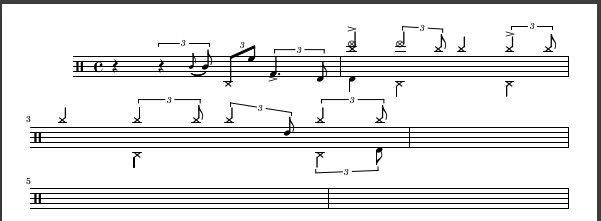
\includegraphics[height=50mm, width=160mm]{z_images/4_experimentations/experience_2/partition.png}\\\\
\textit{En cours…}
\newpage
\subsection*{squant : parsing du fichier midi}
squant lit le midi\\
grammaire wta qui détermine le poid\\
La distance est automatiquement déterminée par squant\\
distance à l’input\\
complexité de la notation

On veut minimiser le coût et la distance $\Rightarrow$ Trouver un compromis.

./build/squant2 -h

Essayer le lire un fichier midi avec squant2
lire mesure par mesure
Regarder les wta(grammaire)

\subsubsection{Quelques tests de lecture midi}
\begin{verbatim}
Les 4 messages suivants sont présents dans tous les tests qui suivent :
[ info] schema file: test/schema/schema-01.wta (??? weight model option)
[warning] no declaration MAX\_GRACE in grammar file test/schema/schema-01.wta
[warning] no declaration TIMESIG in grammar file test/schema/schema-01.wta
[warning] MIDIfile has not joined tracks
\end{verbatim}
./build/squant2 -v 4 -a test/schema/schema-01.wta -m 004\_jazz-funk\_116\_beat\_4-4.mid -config ./params.ini
\begin{verbatim}
[error] at least one of the options -bars or -barsec mandatory
\end{verbatim}
./build/squant2 -verbosity 4 -schema test/schema/schema-01.wta -midi 004\_jazz-funk\_116\_beat\_4-4.mid -config ./params.ini -barsec 3
\begin{verbatim}
squant2: /home/martin/qparselib/src/schemata/SymbLabel.cpp:44: static label_t SymbLabel::make(unsigned char, SymbLabel::Kind, short unsigned int, short unsigned int): Assertion `info2 < 512' failed.
Abandon (core dumped)
\end{verbatim}
Tester squant2 avec le fichiers midi du corpus du gitlab\\\\
La commande suivante :
build/squant2 -v 5 -a ./test/schema/schema-03-R.wta -m ~/corpus-master\_qparselib/103-SaintSaens-elephant/perf/103\_FJ.mid -config ./params.ini -mono -barsec 3.0 -ts 3/4	

Donne :\\
(1) 3($\bullet$, $\overline{2}$:2($\bullet$, ), )\\
(2) 3($\bullet$, $\overline{2}$:2($\bullet$, $\bullet$), )\\
(3) 3($\bullet$, $\overline{2}$:2($\bullet$, $\circ$), )\\\\

% Reste de l’arbre avec des caractères pas encore fonctionnels :
%(4) 3(2̅(2̅(2̅(●, ●), ⏑), ⏑), ⏑:2, )
%(5) 3(2̅(2̅(●, ○), ●), ●:2, )
%(6) 3(2̅(●, 2̅(●, 2̅(○, ●))), ⏑:2, )
%(7) 3(2̅(●, ●), ●:2, )
%(8) 3(2̅(●, 2̅(●, 2̅(⏑, ●))), 2̅(⏑, 2̅(●, ○)), ●)
%(9) 3(●, ●:2, )
%(10) 3(●, 2̅:2(●, 2̅(●, 2̅(⏑, ●))), )
%(11) 3(⏑, 2̅:2(●, ○), )
%(12) 3(●, ⏑, ●)
%(13) 3(●, 2̅:2(2̅(●, 2̅(○, ●)), 2̅(⏑, 2̅(○, ●))), )
%(14) 3(⏑, 2̅:2(●, 2̅(●, ○)), )
%(15) 3(●, ●:2, )
%(16) 3(●, ○:2, )

Pour comprendre les grammaires :\\
Regarder les fichiers wta commentés.\\
https://qparse.gitlabpages.inria.fr/docs/scientific/\\
A\_Parse-based\_Framework\_for\_Coupled\_RhythmQuantization\_and\_Score\_Structuring.pdf
Réfléchir au coût de notation (grace notes, etc.)
\newpage

\subsubsection{cluster.md}
%https://gitlab.inria.fr/qparse/qparselib/-/blob/distance/notes/clusters.md\\\\

\textbf{Caroms of input events}\\

Carom is a synonym for « pileup ». An alternative term could be « cluster » (in the Musical sense, not in the ML sense!).\\

----------------------------------------------------------\\

\textbf{input segment}\\

we assume given in input a sequence of MIDI events $e_0, \ldots, e_n$​​ called "input segment".\\

Every input event is $e_i$ is made of :
\begin{itemize}
	\item an `ON`/`OFF` flag
	\item a MIDI pitch value in $0..127$​
	\item a MIDI velocity value in $0..127$
	\item a date in Real Time Unit (RTU) = seconds, or equivalently MIDI ticks.\\
\end{itemize}

The input events are time-increasing:
$$ date(e_0) \leq  date(e_1) \leq \ldots \leq date(e_n)$$

\textbf{attention:} input event $\neq$​ note (in score):

One input event may have different roles wrt the output score:
\begin{itemize}
	\item begining of note
	\item grace note
	\item trill
	\item end of note
	\item rest
	\item just ignored.\\e.g. in general in MIDI drum input, the `OFF` events will be ignored, but not for piano input.\\
\end{itemize}

----------------------------------------------------------\\

\textbf{Parsing}\\

During parsing, we try several alignements of the input events to particular points in the timeline.\\
The points for alignement are defined by time division, according to a derivation (parse tree) for a CF grammar (actually a tree in a regular tree grammar language).\\

The temporal alignment of an event is done to the point that is the closest to the date of event.
This way, it may happen that several events are aligned to the same point.\\
\newpage

----------------------------------------------------------\\

\textbf{Carom}\\

A carom is a sequence $e_i,\ldots, e_{i+k}$​​ of successive input events (\textit{i.e} a subsequence of the input segment), that ought to be aligned to the same time point. In practice, it is defined by the input segment, $i$ and $k$.\\

Intuitively, it means that the corresponding notes (or rests) will be simultaneous in the output score (e.g. notes in chords, or in different polyphonic voices), or that they will be grace notes.\\

Formally, we define for every transcription case (monophonic instrument, drum, guitar, piano...) a function that depends on the that takes in input\\
\begin{itemize}
	\item a carom $C = e_i,\ldots, e_{i+k}$,
	\item an index $0 \leq j \leq k$,\\
\end{itemize}


and returns the \textit{role} the input event  $e_{i+j}$ in $C$, among:\\
\begin{itemize}
	\item `Ignored`,
	\item `Note`,
	\item `Rest`,
	\item `Staccato`,
	\item `GraceNote`,
	\item `GraceRest`,
	\item maybe more to come...\\
\end{itemize}

For instance, in the case of drum transcription, all `OFF` events are ignored.\\

\textbf{Example 1:}\\\\
In the case of \textbf{drum} transcription, all the pitchs of the following events correspond to the snare-drum (sd).

\begin{table}[h]
\centering
\begin{tabular}{|c|c|c|c|c|}\hline
	event & $e_1$ & $e_2$ & $e_3$ & $e_4$ \\ \hline
	flag & ON & OFF & ON & OFF \\
	pitch & 38 & 38 & 38 & 38 \\ \hline
\end{tabular}	
\end{table}

Therefore we have a sd "flam" (\url{https://en.wikipedia.org/wiki/Drum\_rudiment#Flam}), defined by the following roles:

\begin{table}[h]
	\centering
	\begin{tabular}{|c|c|c|c|c|}\hline
		event & $e_1$ & $e_2$ & $e_3$ & $e_4$ \\ \hline
		role  & GraceNote & Ignored & Note  & Ignored \\ \hline
	\end{tabular}	
\end{table}

We say that $e_3$ is the \textit{main note} associated to (or \textit{decorated by}) the grace note $e_1$.\\

When $e_{i+j}$​ is a grace note ('flam' in the case of drum), we assume moreover a second mapping, called \textit{main}, that associate to $j$​  the index in $[j+1, k]$​ of the corresponding main note.\\

Example 1': in the previous example, $main(1) = 3$.\\



\textbf{Example 2:}\\\\¨
In the case of **monophonic** transcription, the following events: 

| event | $e_1$ | $e_2$ | $e_3$ |
| :---: | :---: | :---: | :---: |
| flag  |  ON   |  OFF  |  ON   |
| pitch |  64   |  64   |  62   |

also correspond to a grace note followed by a note:



| event |   $e_1$   |  $e_2$  | $e_3$ |
| :---: | :-------: | :-----: | :---: |
| role  | GraceNote | Ignored | Note  |



Example 3: still in the case of **monophonic** transcription, for the following events: 

| event | $e_1$ | $e_2$ | $e_3$ |
| :---: | :---: | :---: | :---: |
| flag  |  ON   |  ON   |  OFF  |
| pitch |  64   |  62   |  64   |

we also have the same roles as in Ex.2:



| event |   $e_1$   | $e_2$ |  $e_3$  |
| :---: | :-------: | :---: | :-----: |
| role  | GraceNote | Note  | Ignored |

Indeed, we ignore that fact that the OFF $e_3$ happens  after the ON $e_2$ of next note (e.g. because of the end gesture of the player on the keyboard), because we are in the monophonic case. 



Note that here, we process directly the MIDI input. No pre-processing is assumed, e.g. for eliminating overlaps between the notes 64 and 62. Somehow, elimination of overlaps is ensured by the *role* function for the monophonic case.



Example 4: Back to the case of **drum** transcription, the pitch of $e_1$​​ and $e_2$​ below corresponds to a tom and the one of $e_3, e_4$​ to the sd.

|   event    | $e_1$ | $e_2$ | $e_3$ | $e_4$ |
| :--------: | :---: | :---: | :---: | :---: |
|    flag    |  ON   |  OFF  |  ON   |  OFF  |
|   pitch    |  48   |  48   |  38   |  38   |
| timestamps |  t\_1  |  t\_2  |  t\_3  |  t\_4  |

It could be interpreted either as two simultaneous tom and sd notes, or as a flam between the tom and the sd (the tom is the grace note, the sd the main note). We choose between the two cases according to the "On Tick" distance $t_3 - t_1$.
More precisely, we assume a threshold $\varepsilon$​ such that:

- if $t_3 - t_1 < \varepsilon$​​ then we have 2 simultaneous notes  ("polyphony", between tom and sd, written as a chord):

| event | $e_1$ |  $e_2$  | $e_3$ |  $e_4$  |
| :---: | :---: | :-----: | :---: | :-----: |
| role  | Note  | Ignored | Note  | Ignored |

- if $t_3 - t_1 ≥ \varepsilon$ then we have a flam between tom and sd (written as a grace note):

| event |   $e_1$   |  $e_2$  | $e_3$ |  $e_4$  |
| :---: | :-------: | :-----: | :---: | :-----: |
| role  | GraceNote | Ignored | Note  | Ignored |

The threshold $\varepsilon$ may depend on the latency of an electronic  (MIDI) drum kit used for recording, and/or neuro-acoustic features such as the duration between 2 percussive events above which the perception change from simultaneous, to the phoneme '*flam*'.


\subsubsection{Contributions}

\subsection*{Chaîne de traitement}
\begin{itemize}
	\item Reconnaître un motif (système) sur une mesure de l’input (un fichier midi représentant des données audios)\\ $\Rightarrow$ Motif (système) reconnu : true ou false
	\item Si true : 
	\begin{itemize}
		\item Séparer les voix (\textit{Règles établis par le système})
		\item Simplifier l’écriture de chaque voix (\textit{Règles établis par le système})\\
	\end{itemize}
\end{itemize}

Contribution sur la branch « distance » dans :\\
\begin{itemize}
	\item qparselib/notes/cluster.md
	\item qparselib/src/segment/import/ :\\
	DrumCode hpp et cpp\\
\end{itemize}
\newpage
\section{Résultats et évaluation}
\subsection*{Références pour l’évaluation}
1 - Transcription manuelle à partir de fichier midi et/ou wav d’une partition contenant des systèmes. Écriture des systèmes contenues dans la partition (arbres, séparation des voix, réécriture)
\subsubsection{Comparaison d’arbres}
Trouver un moyen de comparer l’arbre obtenu automatiquement de l’arbre de la transcription manuelle.
\section{Conclusion}
Conclusion de ce chapitre.